\chapter{Simulation Results}

In this chapter, the simulation results for the overall system designed are discussed. And also the behavior of the amplifier for process variation, power supply variation and  temperature variation is discussed. 

\section{DC Analysis}
The test bench to perform the DC analysis is as shown in the Figure.\ref{fig:TB_ACDC}. 

$V_{DD}$ = 2.5V; $V_{SS}$ = -2.5V; $V_{cm}$ = 1.95V; $V_{bias}$ = 150mV to 700mV;  $V_{ac}$ = 1V; $R_{L}$ = 50$\Omega$.
\begin{figure} [H]
\centering
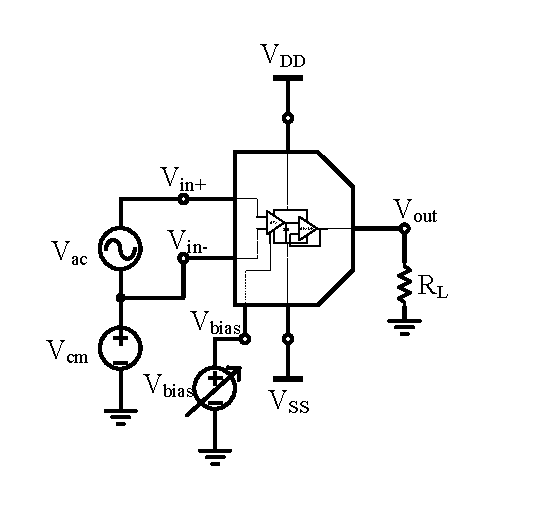
\includegraphics[scale=1]{Figures/Test_Benches/Overall/ACDC.pdf}
\caption{Test setup for DC Analysis}
\label{fig:TB_ACDC}
\end{figure}
The DC Bias point at the output of the system is tabulated in the Table.\ref{tab:DC}. Output DC bias points are almost symmetric around 0V and vary from 180.1mV to -219.3mV.
\begin{table} [H]
\centering
\begin{tabular}{@{}cc@{}}
\toprule
Vbias (mV)			& Output DC Bias (mV)	\\ \midrule
150					& 180.1  \\
200					& 148.4  \\
250					& 115.8  \\
300					& 82.28	 \\
350					& 47.83	 \\
400					& 12.45	 \\
450					& -23.86 \\
500					& -61.08 \\
550					& -99.24 \\
600					& -138.3 \\
650					& -178.4 \\
700 				& -219.3 \\
\bottomrule
\end{tabular}
\caption{DC Bias Point at the output of the circuit}
\label{tab:DC}
\end{table}


\section{AC Analysis}

The test bench in Figure.\ref{fig:TB_ACDC} is used for the AC analysis too. The magnitude of the AC source is set to 1V and as mentioned in the previous chapter, the voltage at the output will be the gain of the overall system.

The plot of gain for different values of $V_{bias}$ is as shown in the Figure.\ref{fig:Gain}. The value of the open loop gain is between 18dB and 25dB.

\begin{figure} [H]
\centering
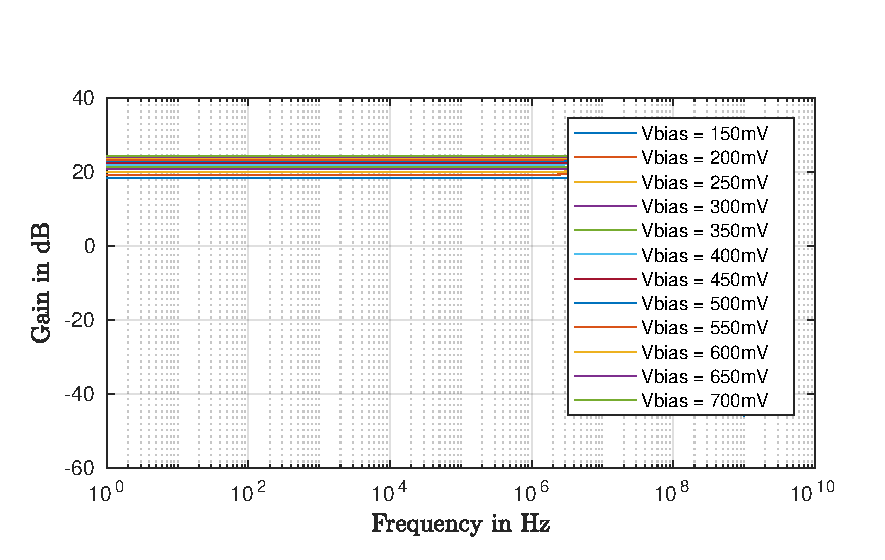
\includegraphics[scale=1]{Figures/Plots/Ov_Gain.pdf}
\caption{Plot of Gain vs Frequency for different Vbias}
\label{fig:Gain}
\end{figure}
The results of the AC analysis are tabulated below in Table.\ref{tab:GAIN_GBW_PM}. The bandwidth is fairly constant at around 14MHz. But the phase margin starting to drop just a tad below 30 with a $V_{bias}$ of 700mV and beyond. 
\begin{table} [H]
\centering
\begin{tabular}{@{}cccc@{}}
\toprule
Vbias (mV)			& DC Gain (dB) 	& Bandwidth (MHz) 	& Phase Margin \\ \midrule
150					& 18.5  		& 14.43 			& 55.49 \\
200					& 19.34			& 14.38 			& 51.37 \\
250					& 20.13  		& 14.34 			& 47.76 \\
300					& 20.83	 		& 14.29 			& 45.08 \\
350					& 21.46			& 14.24 			& 42.55 \\
400					& 22.02	 		& 14.19 			& 40.19 \\
450					& 22.52 		& 14.14 			& 38	\\
500					& 22.97 		& 14.08 			& 35.97	\\
550					& 23.38 		& 14.01 			& 34.08 \\
600					& 23.75 		& 13.95 			& 32.31 \\
650					& 24.1 			& 13.88 			& 30.63 \\
700 				& 24.43 		& 13.8  			& 29.02 \\
\bottomrule
\end{tabular}
\caption{DC Gain, Bandwidth and Phase Margin of the Overall System}
\label{tab:GAIN_GBW_PM}
\end{table}

The test bench in Figure.\ref{fig:TB_ZIN} is used to measure the input impedance of the system. The concept for measurement is same as in the case of the OTA. The voltage at the non-inverting terminal will be the magnitude of the input impedance of the overall system because the magnitude of the current from the AC source is 1A.

$V_{DD}$ = 2.5V; $V_{SS}$ = -2.5V; $V_{bias}$ = 150mV to 700mV;  $I_{sin} magnitude$ = 1A; $R_{L}$ = 50$\Omega$.
\begin{figure} [H]
\centering
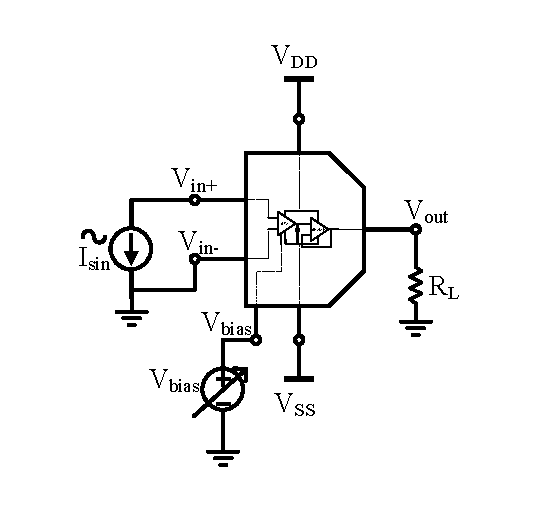
\includegraphics[scale=1]{Figures/Test_Benches/Overall/ZIN.pdf}
\caption{Test setup to measure Input Impedance}
\label{fig:TB_ZIN}
\end{figure}

The value of input impedance with respect to Vbias is tabulated in Table.\ref{tab:ZIN}. It is clear that the input impedance of the overall system is same as the input impedance of the OTA in the first stage.

\begin{table} [H]
\centering
\begin{tabular}{@{}cc@{}}
\toprule
Vbias (mV)			& Input Impedance (M$\Omega$)	\\ \midrule
150					& 3.394  \\
200					& 3.402  \\
250					& 3.41   \\
300					& 3.418	 \\
350					& 3.425	 \\
400					& 3.433	 \\
450					& 3.44  \\
500					& 3.448 \\
550					& 3.456 \\
600					& 3.464 \\
650					& 3.473 \\
700 				& 3.482 \\
\bottomrule
\end{tabular}
\caption{Input Impedance of the Overall System}
\label{tab:ZIN}
\end{table}

On the same lines, the test bench for measuring the output impedance is as shown in the Figure.\ref{fig:TB_ZOUT}. The resistive load is replaced by a current source which tries to pull out 1A of current from the circuit and thereby the voltage at the output turning out to be the magnitude of the output impedance of the system.

$V_{DD}$ = 2.5V; $V_{SS}$ = -2.5V; $V_{cm}$ = 1.95V; $V_{bias}$ = 150mV to 700mV;  $I_{sin} magnitude$ = 1A.
\begin{figure} [H]
\centering
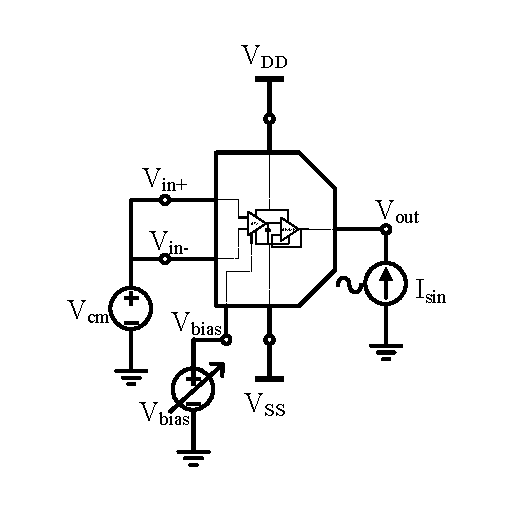
\includegraphics[scale=1]{Figures/Test_Benches/Overall/ZOUT.pdf}
\caption{Test setup to measure Output Impedance}
\label{fig:TB_ZOUT}
\end{figure}

The value of the output impdeance is very low because of the output buffer and there is a small variation of output impedance with change in $V_{bias}$ and is tabulated in Table.\ref{tab:ZOUT}. The values are between 0.94$\Omega$ and 1$\Omega$.
\begin{table} [H]
\centering
\begin{tabular}{@{}cc@{}}
\toprule
Vbias (mV)			& Output Impedance ($\Omega$)	\\ \midrule
150					& 0.9415 \\
200					& 0.9434 \\
250					& 0.9453 \\
300					& 0.9474 \\
350					& 0.9495 \\
400					& 0.9517 \\
450					& 0.9541 \\
500					& 0.9565 \\
550					& 0.9591 \\
600					& 0.9618 \\
650					& 0.9646 \\
700 				& 0.9675 \\
\bottomrule
\end{tabular}
\caption{Output Impedance of the Overall System}
\label{tab:ZOUT}
\end{table}

The next important parameter is the PSRR or the Power Supply Rejection Ratio. It was seen in the previous chapter that the PSRR of the second stage is much more significant than the first stage. Figure.\ref{fig:TB_PSRR} shows the test bench used to measure the PSRR of the whole system. The schematic on the left is used to measure PSRR for $V_{DD}$ and likewise on the right side for $V_{SS}$.

$V_{DD}$ = 2.5V; $V_{SS}$ = -2.5V; $V_{cm}$ = 1.95V; $V_{bias}$ = 150mV to 700mV;  $V_{ac} magnitude$ = 1V; $R_{L}$ = 50$\Omega$.

\begin{figure} [H]
\centering
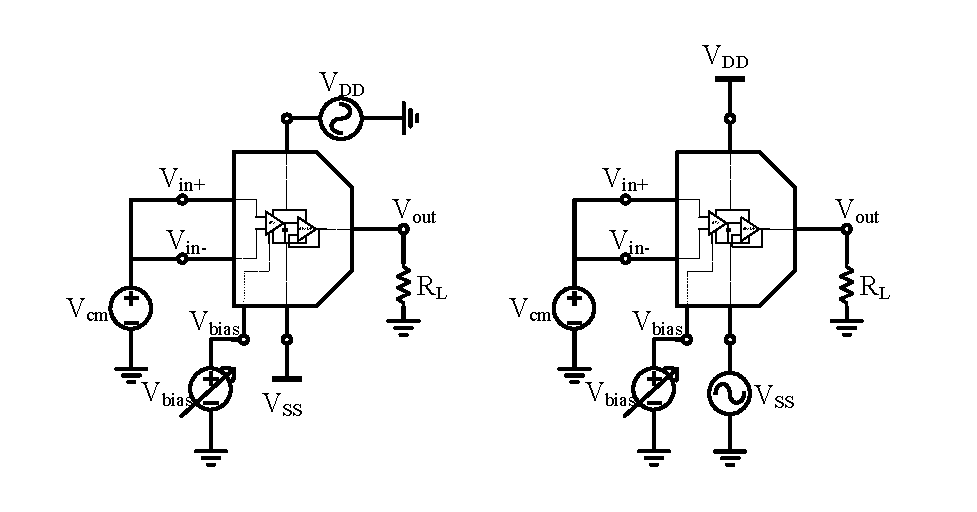
\includegraphics[scale=1]{Figures/Test_Benches/Overall/PSRR.pdf}
\caption{Test setup to measure PSRR}
\label{fig:TB_PSRR}
\end{figure}

The variation of PSRR against $V_{bias}$ is tabulated below in Table.\ref{tab:PSRR}. PSRR is high for high bias currents or low values of $V_{bias}$ and it decreases with increase in $V_{bias}$. PSRR is generally expressed in terms of dB. But from the specifications, it is seen that the parameter has to be expressed in uA/V as part of this work.

\begin{table} [H]
\centering
\begin{tabular}{@{}ccc@{}}
\toprule
Vbias (mV)			& PSRR (VDD)(uA/V)			& PSRR (VSS)(uA/V)	 \\ \midrule
150					& 97.76	 					& 93.69					 \\
200					& 89.66 					& 85.77					 \\
250					& 82.86 					& 79.11					 \\
300					& 77.26 					& 73.59					 \\
350					& 72.68						& 69.04					 \\
400					& 68.93						& 65.28					 \\
450					& 65.84 					& 62.18					 \\
500					& 63.27						& 59.53					 \\
550					& 61.1	 					& 57.26					 \\
600					& 59.22 					& 55.28					 \\
650					& 57.59 					& 53.52					 \\
700 				& 56.13 					& 51.92					 \\
\bottomrule
\end{tabular}
\caption{PSRR of the Overall System}
\label{tab:PSRR}
\end{table}

\section{Transient Analysis}
The transient analysis is divided in to two parts. The first part involves simulation with a sine wave input and the second part involves simulation with a square wave input. The test bench for transient analysis with a sine wave input for the system is as shown in Figure.\ref{fig:TB_SINE}.

$V_{DD}$ = 2.5V; $V_{SS}$ = -2.5V; $V_{cm}$ = 1.95V; $V_{bias}$ = 150mV to 700mV;  $V_{sin} amplitude$ = 100mV; $R_{L}$ = 50$\Omega$.

\begin{figure} [H]
\centering
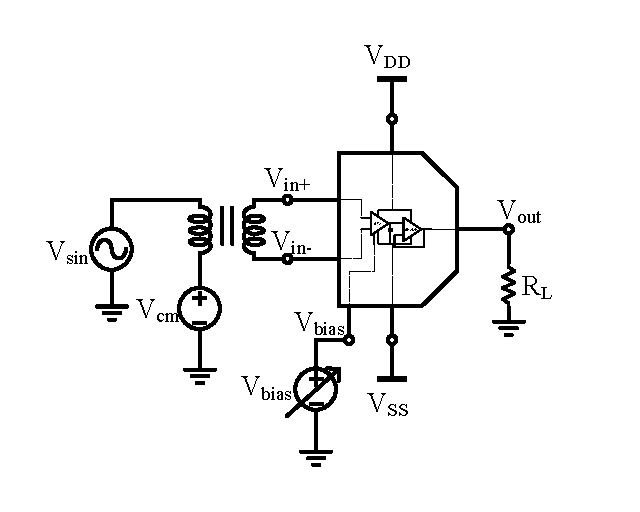
\includegraphics[scale=1]{Figures/Test_Benches/Overall/SINE.pdf}
\caption{Test setup for Transient Analysis - Sine Wave input}
\label{fig:TB_SINE}
\end{figure}

The plot of output current against time for different values of $V_{bias}$ is as shown in the Figure.\ref{fig:SINE}. The peaks are not symmetric around zero, however it is made sure that the peak-to-peak current values range from 30mA to 60mA.

\begin{figure} [H]
\centering
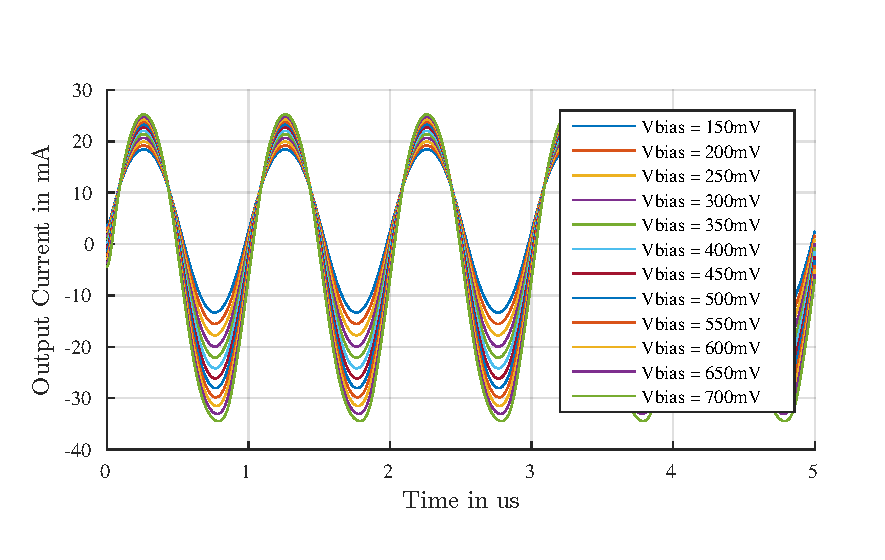
\includegraphics[scale=1]{Figures/Plots/Ov_Sine_Iout.pdf}
\caption{Plot of Output Current vs time for different Vbias}
\label{fig:SINE}
\end{figure}

Table.\ref{tab:SINE} gives a better picture of the sinusoidal plots shown above. The HD2 and HD3 values are less than 30 dBc. However, the HD3 seems to take a turn towards the worse with increase in $V_{bias}$. So for $V_{bias}$ values beyond 700mV, the output starts clipping at the trough of the current wave.

\begin{table} [H]
\centering
\begin{tabular}{@{}cccccc@{}}
\toprule
Vbias (mV)		& Iout Max(mA)		& Iout Min(mA)	 & Iout p2p(mA) & HD2 (dBc)	&HD3 (dBc) \\ \midrule
150				& 18.43	 			& -13.34		 & 31.77		& -37.14		& -48.17	\\
200				& 19.17 			& -15.55		 & 34.72		& -36.62		& -45.67	\\
250				& 19.93 			& -17.77		 & 37.7			& -35.65		& -43.65	\\
300				& 20.67 			& -19.97		 & 40.64		& -35.15		& -42.07	\\
350				& 21.38				& -22.12		 & 43.49		& -34.84		& -40.83	\\
400				& 22.04				& -24.19		 & 46.23		& -34.72		& -39.85	\\
450				& 22.66 			& -26.17		 & 48.83		& -34.8			& -39.01	\\
500				& 23.24				& -28.05		 & 51.29		& -35.08		& -38.24	\\
550				& 23.77	 			& -29.83		 & 53.6			& -35.54		& -37.42	\\
600				& 24.28 			& -31.51		 & 55.79		& -36.13		& -36.47	\\
650				& 24.76 			& -33.07		 & 57.83		& -36.61		& -35.24	\\
700 			& 25.24 			& -34.47		 & 59.71		& -36.44		& -33.61	\\
\bottomrule
\end{tabular}
\caption{Transient Parameters of the Overall System}
\label{tab:SINE}
\end{table}

Once the peak-to-peak value of current is obtained, we can use that to calculate the transconductance of the system for different $V_{bias}$ values. Transconductance is the ratio of output current to the input voltage. Since the output current is not symmetric around 0A, the the value half of peak-to-peak current is considered. That divided by the input voltage (100mV peak) would give us the required transconductance value. Figure.\ref{fig:GM} shows the plot of transconductance against $V_{bias}$. And it rightfully follows the behavior of the output current.

\begin{figure} [H]
\centering
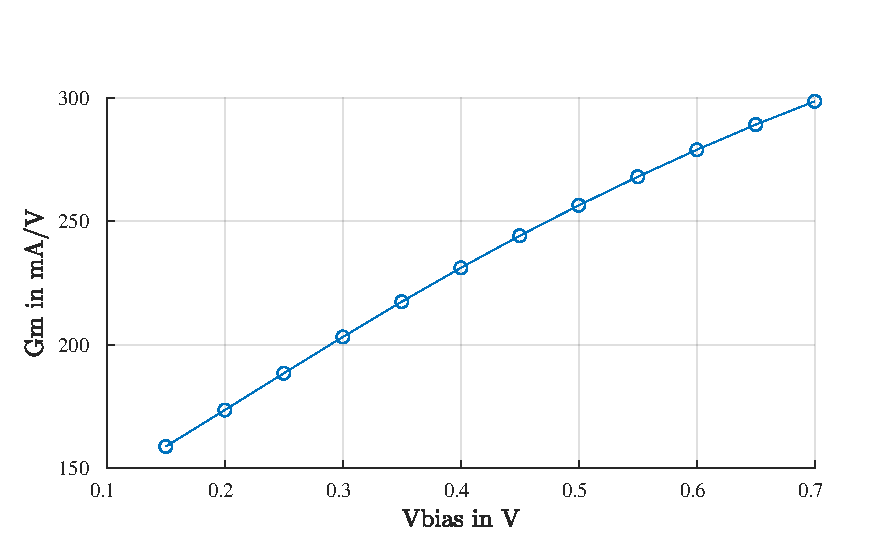
\includegraphics[scale=1]{Figures/Plots/Ov_Gm.pdf}
\caption{Plot of Gm vs Vbias}
\label{fig:GM}
\end{figure}

The transconductance value for each $V_{bias}$ used to plot the Figure.\ref{fig:GM} is tabulated in Table.\ref{tab:GM}.

\begin{table} [H]
\centering
\begin{tabular}{@{}cc@{}}
\toprule
Vbias (mV)			& Transconductance (mA/V)	\\ \midrule
150					& 158.8 \\
200					& 173.6 \\
250					& 188.5 \\
300					& 203.2 \\
350					& 217.5 \\
400					& 231.2 \\
450					& 244.2 \\
500					& 256.4 \\
550					& 268 \\
600					& 278.9 \\
650					& 289.1 \\
700 				& 298.5 \\
\bottomrule
\end{tabular}
\caption{Transconductance Gain of the Overall System}
\label{tab:GM}
\end{table}

Now, the second part of the transient analysis is performed with a square wave input. Figure.\ref{fig:TB_SLEW} shows the test bench for transient analysis for a square wave input. The system is connected in a unity gain configuration.

\begin{figure} [H]
\centering
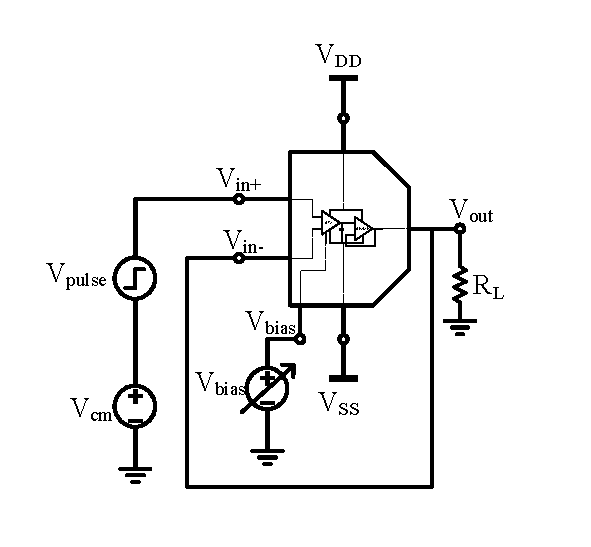
\includegraphics[scale=1]{Figures/Test_Benches/Overall/SLEW.pdf}
\caption{Test setup for Transient Analysis - Square Wave input}
\label{fig:TB_SLEW}
\end{figure}
The slew rate for the rising edge and the falling edge is tabulated in the Table.\ref{tab:SLEW}. The slew rate is at a low value due to the fact that the OP AMP designed exhibits a very low slew rate.
 
\begin{table} [H]
\centering
\begin{tabular}{@{}ccc@{}}
\toprule
Vbias (mV)			& Slew Rate (Rising Edge)(V/us)			& Slew Rate (Falling Edge)(V/us)	 \\ \midrule
150					& 6.985	 					& -8.73					 \\
200					& 7.505 					& -9.779				 \\
250					& 8.042 					& -10.68				 \\
300					& 8.581 					& -11.34				 \\
350					& 9.095						& -11.66				 \\
400					& 9.561						& -11.7					 \\
450					& 9.954 					& -11.6					 \\
500					& 10.27						& -11.45				 \\
550					& 10.49	 					& -11.3					 \\
600					& 10.65 					& -11.14				 \\
650					& 10.76 					& -10.99				 \\
700 				& 10.82 					& -10.84				 \\
\bottomrule
\end{tabular}
\caption{Slew Rate of the Overall System}
\label{tab:SLEW}
\end{table}

\section{Noise Analysis}
The test bench to perform the noise analysis is same as the test bench used for AC analysis in Figure.\ref{fig:TB_ACDC}. The input referred noise of the first stage is far more significant for the overall system than the second stage.

The Bode plot of the input referred noise for different values of $V_{bias}$ is shown in the Figure.\ref{fig:NOISE}. It is clear that the type of noise is 1/f noise or the Flicker noise. The magnitude of the input referred noise is very high for low frequencies and it reduces significantly in moderate and high frequencies when White noise starts to dominate.

\begin{figure} [H]
\centering
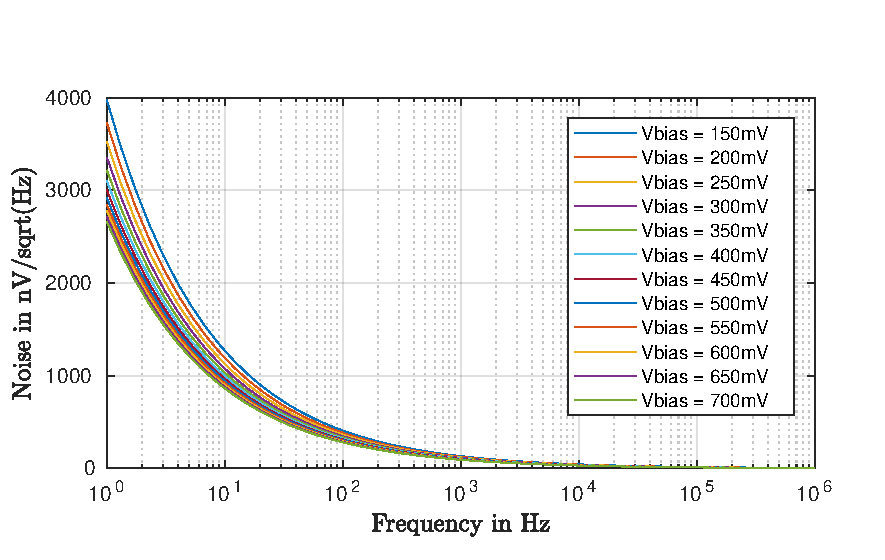
\includegraphics[scale=1]{Figures/Plots/Ov_Noise.pdf}
\caption{Plot of Input Referred Noise vs Frequency for different Vbias}
\label{fig:NOISE}
\end{figure}

The value of input referred noise at 1MHz for different $V_{bias}$ is tabulated in the Table.\ref{tab:NOISE}.

\begin{table} [H]
\centering
\begin{tabular}{@{}cc@{}}
\toprule
Vbias (mV)			& Input Referred Noise (nV/sqrt(Hz))	\\ \midrule
150					& 46.64 \\
200					& 43.93 \\
250					& 41.71 \\
300					& 39.91 \\
350					& 38.46 \\
400					& 37.29 \\
450					& 36.33 \\
500					& 35.52 \\
550					& 34.82 \\
600					& 34.21 \\
650					& 33.66 \\
700 				& 33.16 \\
\bottomrule
\end{tabular}
\caption{Input Referred Noise of the Overall System}
\label{tab:NOISE}
\end{table}


\section{Programmable Load}
Another way to make the overall system programmable is to have a programmable load. Having a Resistive load that varies would imply that the current flowing through the load is controlled. So, for the following analyses, the $V_{bias}$ is made constant and set a value of 425mV.

Table.\ref{tab:RL_AC_1} shows the variation of DC Gain, bandwidth, phase margin and transconductance with varying load. The gain hadly changes with the changing load. The variation in bandwidth is just 1.8MHz between the minimum and maximum load. The transconductance however, shows variation in a range that is expected.
 
\begin{table} [H]
\centering
\begin{tabular}{@{}ccccccc@{}}
\toprule
RL ($\Omega$)		& DC Gain(dB)		& Bandwidth(MHz)		& Phase Margin			& Transconductance(mA/V)\\ \midrule
35		& 22.2 		& 13.13		& 40.97		& 338.9		\\
40		& 22.22 	& 13.55		& 40.22		& 296.8		\\
45		& 22.25 	& 13.88		& 39.6		& 264		\\
50		& 22.28 	& 14.16		& 39.08		& 237.7		\\
55		& 22.3 		& 14.4		& 38.63		& 216.2		\\
60		& 22.32 	& 14.6		& 38.24		& 198.3		\\
65		& 22.34 	& 14.77		& 37.9	 	& 183.1		\\
70		& 22.35 	& 14.92		& 37.6		& 170		\\
\bottomrule
\end{tabular}
\caption{AC Parameters of the Overall System for a programmable load - 1}
\label{tab:RL_AC_1}
\end{table}

Table.\ref{tab:RL_AC_2} shows the tabulation of values for the parameters that are independent of the variation in load resistance.

\begin{table} [H]
\centering
\begin{tabular}{@{}cc@{}}
\toprule
Parameter							& Value		\\ \midrule
Input Impedance M($\Omega$)			& 3.436 	\\
Output Impedance ($\Omega$)			& 0.953 	\\
PSRR (VDD)(uA/V)					& 67.32 	\\
PSRR (VSS)(uA/V)					& 63.65 	\\
Input Referred Noise (nV/$\sqrt{Hz}$)	& 36.79		\\
\bottomrule
\end{tabular}
\caption{AC Parameters of the Overall System for a programmable load - 2}
\label{tab:RL_AC_2}
\end{table}

The transient analysis of the system with a programmable load shows a clear picture of how effective the system is. Since the bias voltage or the bias current doesn't change, the DC bias point at the output of the system remains unchanged. Therefore, we get a symmetrical waveform around 0A. The plot in Figure.\ref{fig:RL_SINE} shows the output current plot for different values of load resistance. 
\begin{figure} [H]
\centering
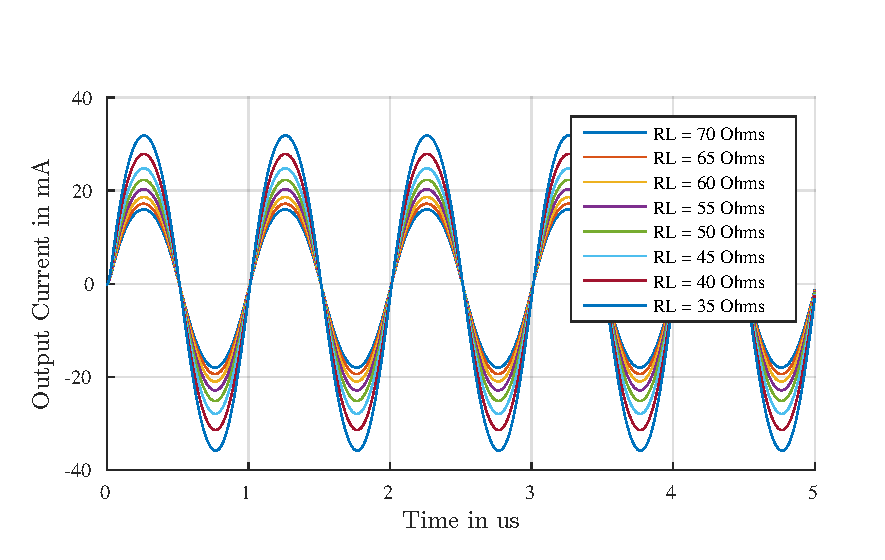
\includegraphics[scale=1]{Figures/Plots/Ov_Sine_RL.pdf}
\caption{Plot of Output Current vs Time for different RL}
\label{fig:RL_SINE}
\end{figure}
Table.\ref{tab:RL_trans_1} contains tabulation from the plot in Figure.\ref{fig:RL_SINE}. Output current is the most significant parameter that gets affected by a variable load.
\begin{table} [H]
\centering
\begin{tabular}{@{}cccc@{}}
\toprule
RL ($\Omega$)			& Iout(max)(mA)		& Iout(min)(mA)		& Iout(p2p)(mA) \\ \midrule
35					& 31.89 			& -35.89			& 67.77			\\
40					& 27.92 			& -31.44			& 59.36			\\
45					& 24.83 			& -27.97			& 52.8			\\
50					& 22.36 			& -25.19			& 47.55			\\
55					& 20.33 			& -22.91			& 43.24			\\
60					& 18.65 			& -21.01			& 39.65			\\
65					& 17.22 			& -19.4				& 36.61 		\\
70					& 15.99 			& -18.02			& 34.01			\\
\bottomrule
\end{tabular}
\caption{Maximum and Minimum Output Currents for a programmable load}
\label{tab:RL_trans_1}
\end{table}

Table.\ref{tab:RL_trans_2} shows the values of the parameters that are constant with a varying load. HD2 and HD3 are less than -30dBc.
\begin{table} [H]
\centering
\begin{tabular}{@{}cc@{}}
\toprule
Parameter							& Value		\\ \midrule
HD2 (dBc)							& -34.6 			\\
HD3 (dBc)							& -39.4 			\\
Slew Rate (Rising Edge)(V/us)		& 10.28 			\\
Slew Rate (Falling Edge)(V/us)		& -10.45 			\\
\bottomrule
\end{tabular}
\caption{Transient Parameters of the Overall System for a programmable load}
\label{tab:RL_trans_2}
\end{table}
And finally, we have the plot of transconductance versus the load resistance as shown in Figure.\ref{fig:RL_Gm}
\begin{figure} [H]
\centering
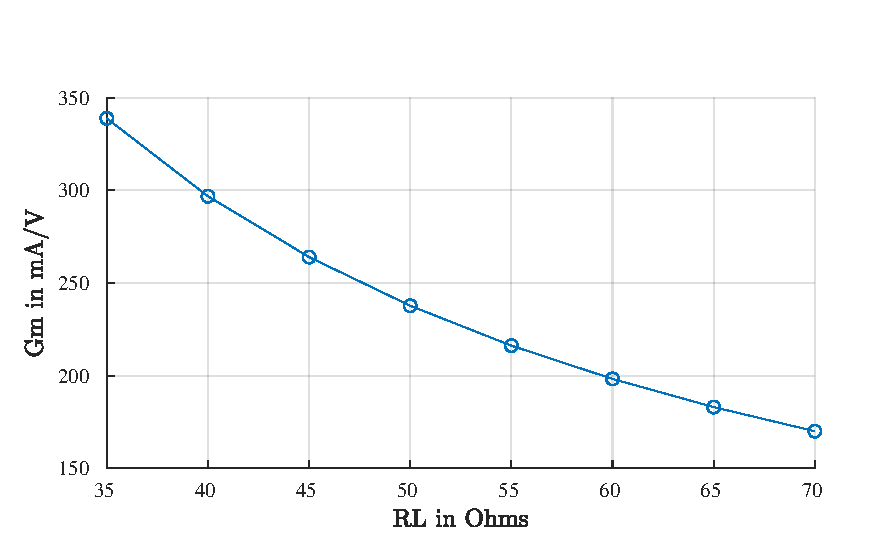
\includegraphics[scale=1]{Figures/Plots/Ov_Gm_RL.pdf}
\caption{Plot of Transconductance vs RL}
\label{fig:RL_Gm}
\end{figure}

\section{Corner Simulation}
\subsection{Process Variation}
\subsection{Process and Supply Variation}
\subsection{Process, Voltage and Temperature (PVT) variation}
\subsection{Summary of PVT Corner Analysis}